%####################################################
\section{Importance sampling and Sequential Monte Carlo}
%####################################################
\subsection{Importance sampling : basics}
%####################################################
\begin{frame}[allowframebreaks]\frametitle{Importance sampling}
%####################################################


\begin{itemize}


\item For any function  $\varphi$ (...), $$E_{\theta | \bY} [\varphi(\theta)] = \int_\Theta \varphi(\theta) \vert \pi(\theta|\bY) d\theta\noir = \int_\Theta \varphi(\theta) \frac{\pi(\theta|\bY)}{\eta(\theta)}\vert \eta(\theta) d\theta\noir  $$
\item with  $\eta$ easily simulable distribution, such that its support contains the one of $\pi(\theta|\bY)$,  whose density can be computed.  
\end{itemize} 
 \framebreak
 

\vert  Monte Carlo estimator \noir  : $\theta^{(1)}, \dots , \theta^{(M)} \sim_{i.i.d.} \eta$
 
\begin{eqnarray*}
\widehat{E}_n[\varphi(\theta)] &=& \frac{1}{M}  \sum_{m=1}^M \frac{\pi(\theta^{(m)}| \bY)}{\eta(\theta^{(m)})}   \varphi(\theta^{(m)})\\&=&   \frac{1}{M}  \frac{1}{p(\bY)} \sum_{m=1}^M   \underbrace{\frac{ \ell(\bY | \theta^{(m)}) \pi(\theta^{(m)})}{ \eta(\theta ^{(m)})}}_{w^{(m)} }  \varphi(\theta^{(m)}) 
\end{eqnarray*}
 \vert But \noir  $p(\bY) $ without explicit expression:  $$p(\bY)  = \int  \ell(\bY | \theta) \pi(\theta)d\theta = \int \frac{ \ell(\bY | \theta) \pi(\theta)}{\eta(\theta)} \eta(\theta)d\theta  $$
$$\widehat{p(\bY)} =\frac{1}{M} \sum_{m=1}^n\frac{ \ell(\bY | \theta^{(m)}) \pi(\theta^{(m)})}{\eta(\theta ^{(m)})}  = \frac{1}{M}\sum_{m=1}^N w^{(m)}$$

  \begin{eqnarray*}
\widehat{E}_{\theta|\bY}[\varphi(\theta)] &=&  \frac{1}{M}  \sum_{m=1}^M  \frac{w^{(m)}}{p(\bY)} \varphi(\theta^{(m)})\\
\widehat{\widehat{E}}_{\theta | \bY} [\varphi(\theta)] &=& \frac{\cancel{\frac{1}{M}}  \sum_{m=1}^M  \rouge w_n^{(m)} \noir \varphi(\theta^{(m)})} { \cancel{\frac{1}{M}}  \rouge \sum_{m=1}^M  w^{(m)} \noir}\\
&=&   \sum_{m=1}^M  W^{(m)}  \varphi(\theta^{(m)})   \mbox{ avec } W^{(m)} = \frac{w^{(m)}}{ \sum_{m=1}^M w^{(m)}} 
\end{eqnarray*}
\begin{center}\vert Consistant Estimator \end{center}
\end{frame}

%####################################################
\begin{frame}\frametitle{Importance Sampling}
%####################################################

\begin{block}{Summary}
 Approximate $\pi(\theta | \bY)$ by a weighted sample $(\theta^{(m)}, W^{(m)})_{m=1\dots M}$ such that
$$ \theta^{(m)} \sim_{i.i.d.} \eta(\cdot)$$ 
$$W^{(m)} = \frac{w^{(m)}}{ \sum_{m=1}^M w^{(m)}}$$
$$ w^{(m)} = \frac{ \ell(\bY | \theta^{(m)}) \pi(\theta^{(m)})}{ \eta(\theta ^{(m)})}$$
\end{block}
\end{frame}


%####################################################
\begin{frame}{Importance Sampling: example}
%####################################################

\centering
 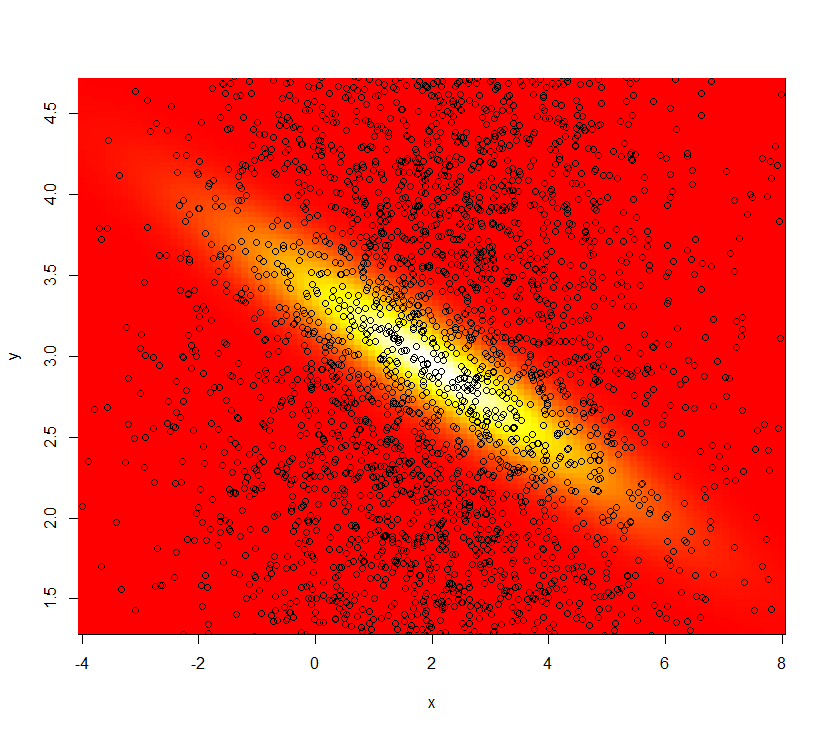
\includegraphics[width=0.8\textwidth]{figures/IS_sampling.png}
 
 Simulated particles, without their weights
 \end{frame}

 
%####################################################
 \begin{frame}{Importance Sampling: posterior}
%####################################################
 
\begin{figure}
   \begin{minipage}[c]{.46\linewidth}
 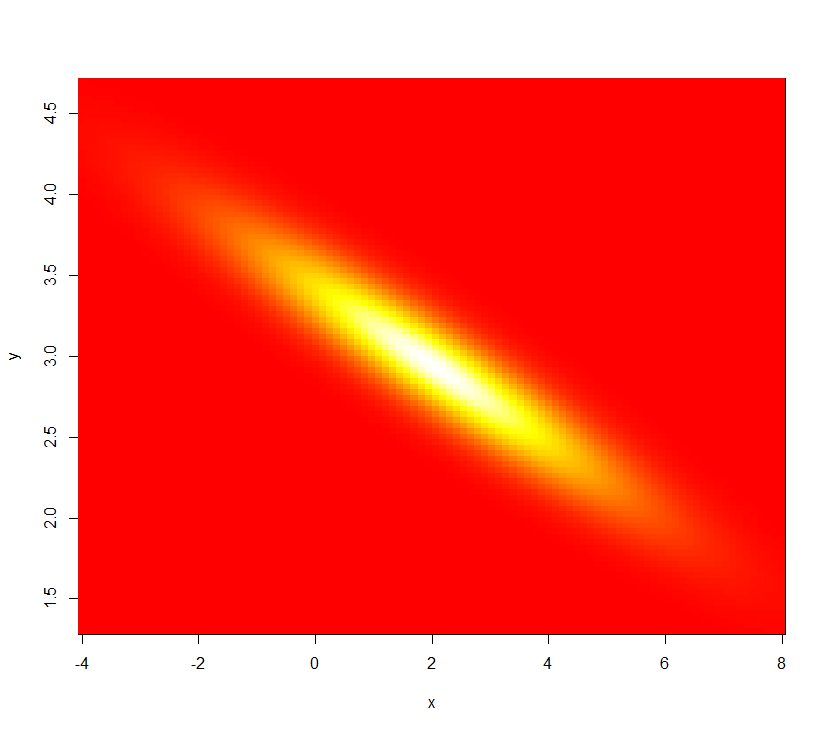
\includegraphics[width=\textwidth]{figures/post_2D_true.png}
   \end{minipage} \hfill
   \begin{minipage}[c]{.46\linewidth}
  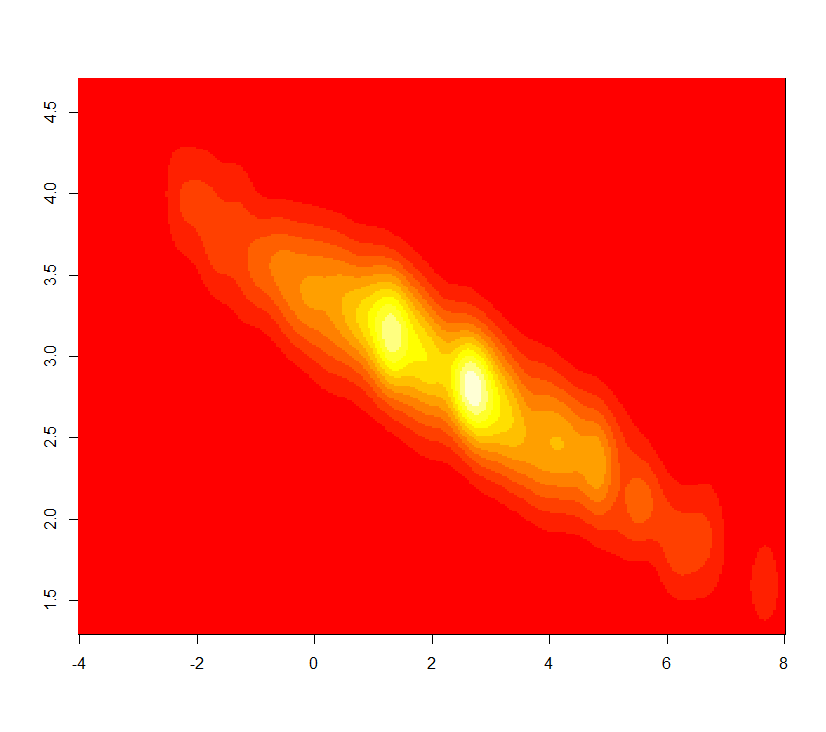
\includegraphics[width=\textwidth]{figures/post_2D_IS.png}
   \end{minipage}
   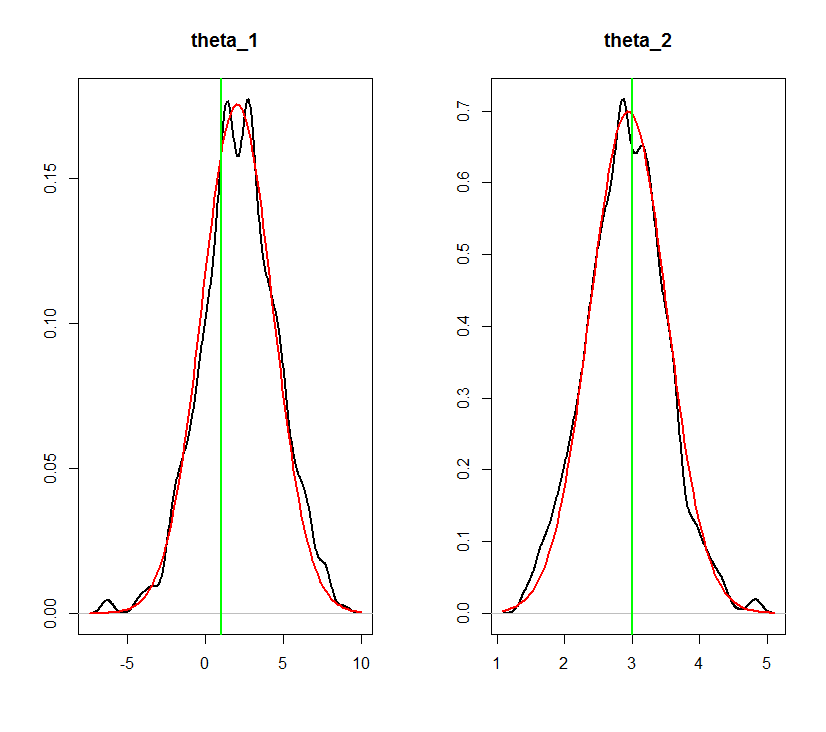
\includegraphics[width=\textwidth,height=3.8cm]{figures/post_IS_vraie.png}
\end{figure}
\end{frame}

%####################################################
\begin{frame}{Importance Sampling: an example that does not work}
%####################################################

\centering
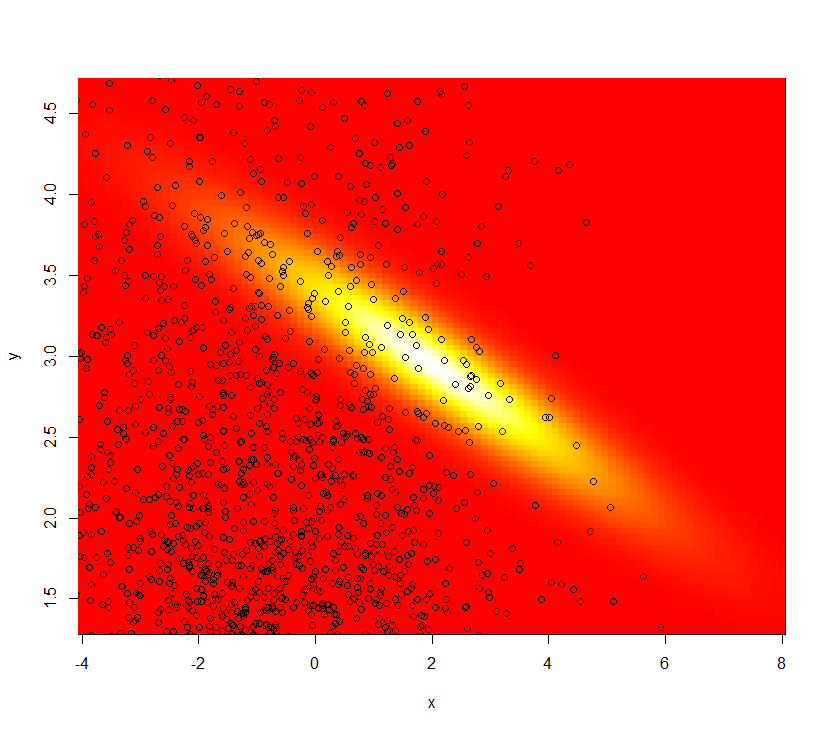
\includegraphics[width=0.8\textwidth]{figures/IS_sampling_2.png}
 
Simulated particles, without their weights 
\end{frame}

 
%####################################################
\begin{frame}{Importance Sampling: un example that does not work}
%####################################################
\begin{figure}
   \begin{minipage}[c]{.46\linewidth}
 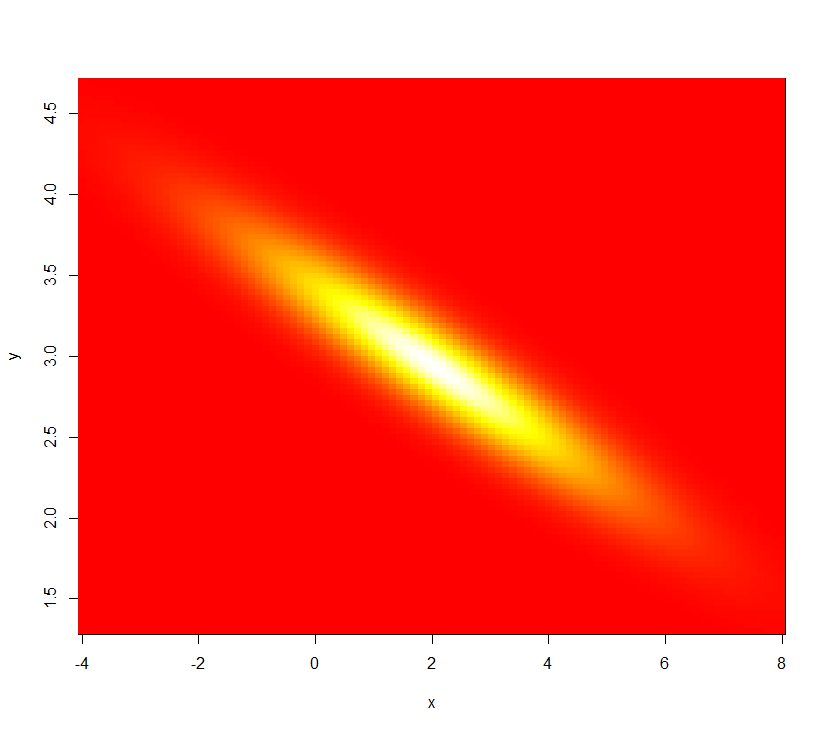
\includegraphics[width=\textwidth]{figures/post_2D_true.png}
   \end{minipage} \hfill
   \begin{minipage}[c]{.46\linewidth}
  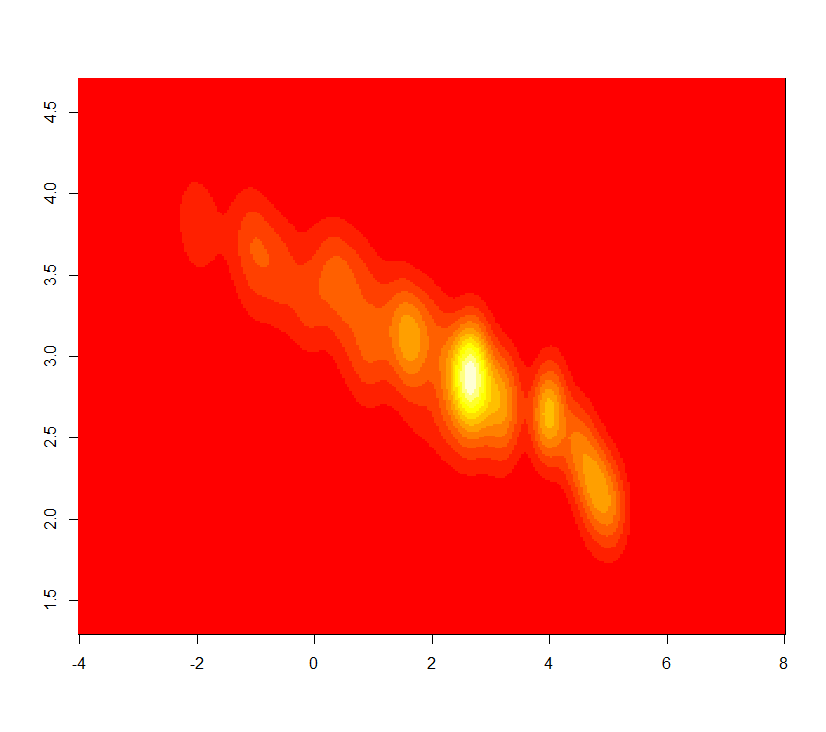
\includegraphics[width=\textwidth]{figures/post_2D_IS_2.png}
   \end{minipage}
   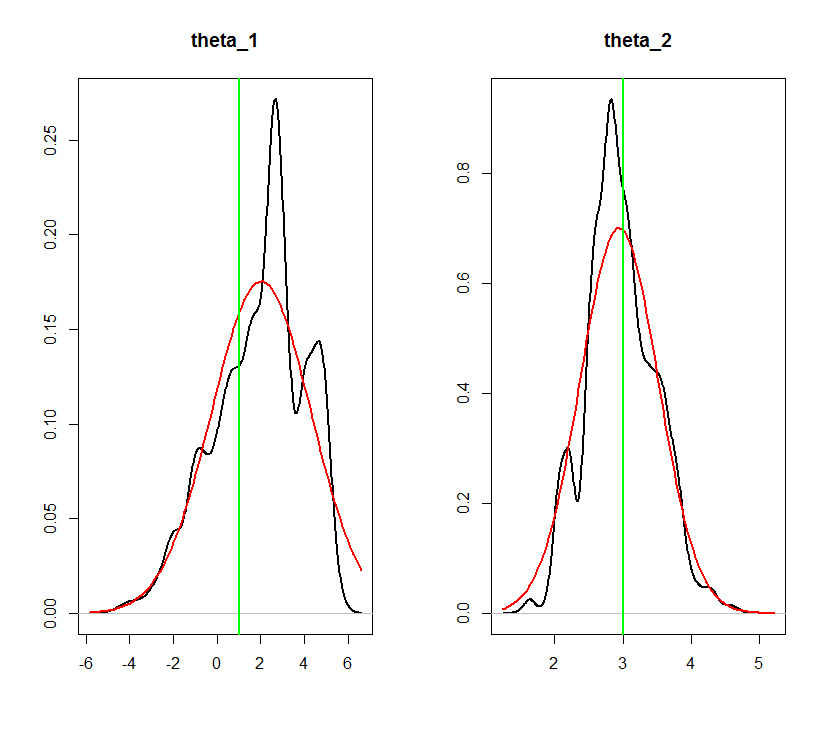
\includegraphics[width=\textwidth,height=3.8cm]{figures/post_IS_vraie_2.png}
\end{figure}
\end{frame}



%####################################################
 \begin{frame}[allowframebreaks=0.8]{Importance sampling methods: comments}
%####################################################

\begin{itemize}
\item Convergence ensured by the large numbers law. 
\item But the quality of the estimator (variance) for a given $M$ ?   
\item  Problem if some weights are very large while others are very small. 
\begin{itemize}
\item Calculus of the \vert Effective Sample Size\noir: 
$$ ESS = \frac{1}{ \sum_{m=M}^N \left(W^{(m)}\right)^2 }$$
\item $EES \in [1,M]$. 
\item The weighted sample $(W^{(m)},  \theta^{(m)})$  corresponds to a no-weighted sample of size  $ESS$ 
\end{itemize}
\item Essential to chose  $\eta$ carefully such that   $\ell(\bY| \theta^{(m)}) \pi(\theta^{(m)})$ not two small. 
\item Not possible in large dimension problems: need to sequentially build $\eta$ \vert Sequential Monte Carlo \noir
\item \vert Advantage: \noir easy estimation of $p(\bY)$ par $\sum_{m=1}^M w^{(m)}$
\end{itemize}
\end{frame}

%####################################################
\subsection[VB-IS]{Sequential Importance Sampling}
%####################################################
\begin{frame}\frametitle{}
%####################################################


\begin{block}{Problematic}
Can we use the variational approximation of the posterior distribution in a IS procedure. Can we correct its tendancy to under-estimate the posterior variance?  
\end{block}

Let  $\eta^{VB}$ be the VB posterior approximation of  $\pi(\theta|\bY)$. 

\begin{block}{Naive idea}
\begin{itemize}
\item IS using  $\eta_{VB}$ as a sampling distribution
\item  \vert But\noir : $\eta_{VB}$ has a support smaller than the one of  $\pi(\theta|\bY)$ 
\end{itemize}
\end{block}
\begin{block}{Naive idea 2}
\begin{itemize}
\item Using a dilated version of  $\eta_{VB}$
\item  Problems : how? how much? 
\item The problems of neglected dependencies remains
\end{itemize}
\end{block}

\end{frame}
%####################################################
\begin{frame}{IS with $\eta_{VB}$ }
%####################################################

\centering 
 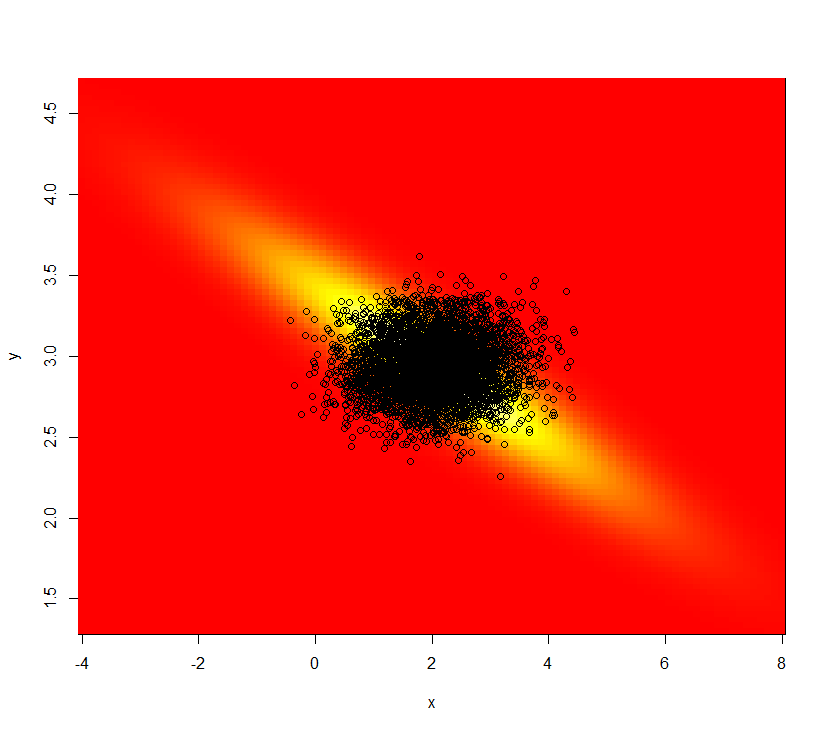
\includegraphics[width=0.8\textwidth]{figures/IS_sampling_VBEM.png}
 
 Particles simulated not weighted 
  \end{frame}
 %----------------------------------------------------------------------

%####################################################
\begin{frame}{IS with $\eta_{VB}$}
%####################################################

\begin{figure}
   \begin{minipage}[c]{.46\linewidth}
 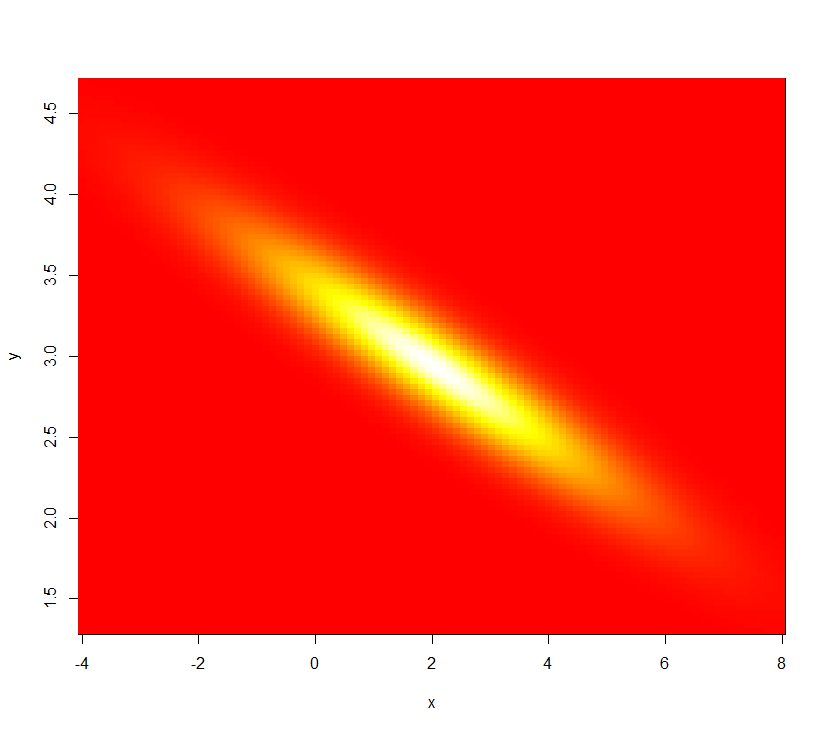
\includegraphics[width=\textwidth]{figures/post_2D_true.png}
   \end{minipage} \hfill
   \begin{minipage}[c]{.46\linewidth}
  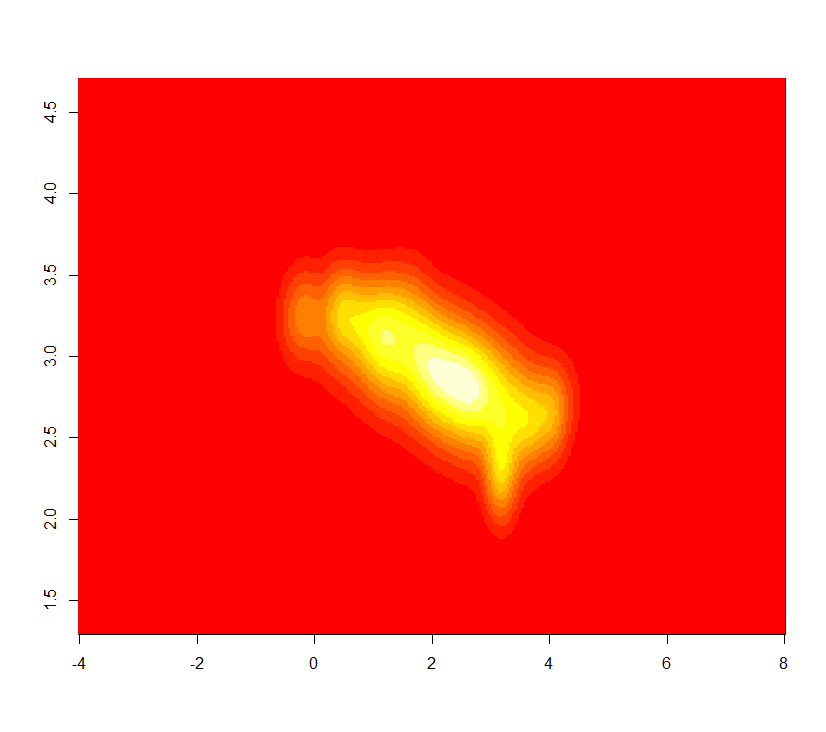
\includegraphics[width=\textwidth]{figures/post_2D_IS_VBEM.png}
   \end{minipage}
   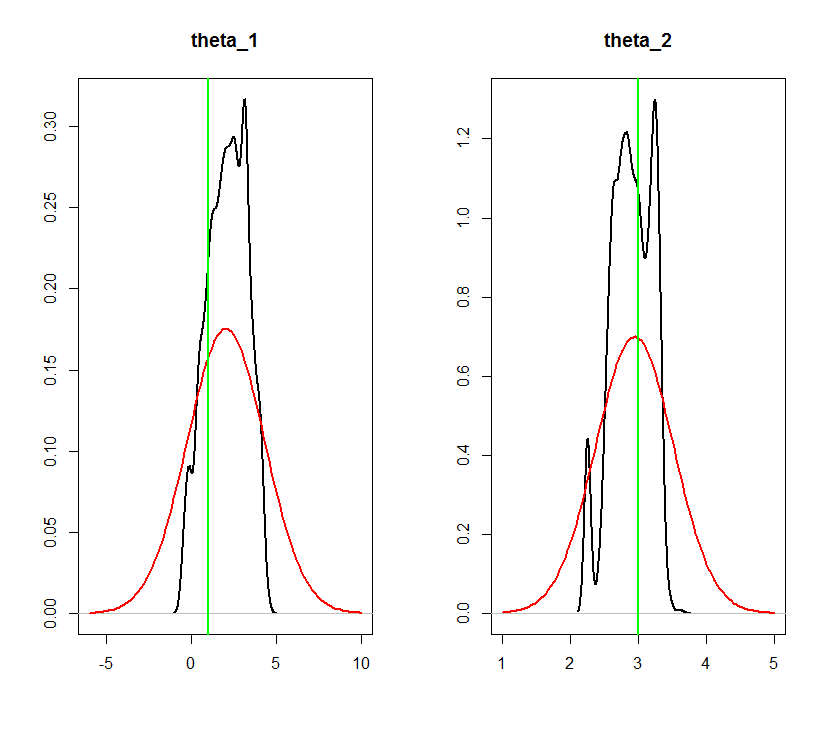
\includegraphics[width=\textwidth,height=3.5cm]{figures/post_IS_vraie_VBEM.png}
\end{figure}
\end{frame}



%####################################################
\begin{frame}\frametitle{One solution}
%####################################################


\begin{block}{Sequential sampling of a sequence of distributions} 
Let $\alpha_n$ be a increasing sequence such that
$\alpha_0 = 0  $ et $\alpha_N=1 $. 

Sample sequentially 
$$\pi_n(\theta)  \propto   \eta_{VB}(\theta)^{1- \alpha_n} (\ell(\bY | \theta) \pi(\theta))^{\alpha_n} = \frac{\gamma_n(\theta)}{Z_n}$$ 
using at each step  $n$  a sampling distribution  $\eta_n$ ``judicious''. 
\end{block}

\vert Remarks: \noir
\begin{itemize}
\item $\log\pi_n(\theta) = Cste +   (1- \alpha_n)  \log \eta_{VB}(\theta) + \alpha_n  \log (\ell(\bY | \theta) \pi(\theta))$
\item $n=0$ : $\pi_n(\theta)   =   \eta_{VB}(\theta)$.  Easy to simulate.  
\item $n=N$ : $ \pi_n(\theta)   \propto   \ell(\bY | \theta) \pi(\theta) = \pi(\theta| \bY)$: \vert goal reached
\item If $\alpha_n$ does not increase too fast $\pi_n(\theta) \approx \pi_{n+1}(\theta)$. 
 \end{itemize}
\end{frame}




%####################################################
\begin{frame}\frametitle{From $\eta_n$ to $\eta_{n+1}$}
%#################################################### 
 Assume that at itération $n$,  we have built  $\eta_n$ efficient for  $\pi_n$ :  $$\theta_n^{(1)}, \dots, \theta_n^{(M)} \sim \eta_n(\theta)$$ 
\vspace{1em}

At iteration  $n+1$,  we want to simulate  $\pi_{n+1}(\theta)$ using that previous sample
\begin{itemize}
\item \vert Intuition \noir: if $\pi_n \approx \pi_{n+1}$ simulate $\theta_{n}^{(m)}$ in a neighbourood of  $\theta_{n+1}^{(m)}$, i.e. using a Markovian kernel
$$ \theta_{n+1}^{(m)} | \theta_n^{(m)} \sim K_{n+1}(\theta_n^{(m)}, \theta_{n+1}^{(m)})$$
\item[] Example : $ \theta_{n+1}^{(m)} = \theta_n^{(m)} + \varepsilon_i$ with $\varepsilon_i \sim\mathcal{N}(0,\rho^2)$ 
\item  \vert New weights: \noir  $$w_{n+1}(\theta) = \frac{\gamma_{n+1}(\theta)}{\eta_{n+1}(\theta)} $$

\item \vert But \noir 
$$\eta_{n+1}(\theta_{n+1})  = \int_{\Theta}\eta_n(\theta_n) K _{n+1}(\theta_n,\theta_{n+1}) d\theta_n$$

\begin{center}
No explicit expression
\end{center}
\end{itemize}

\end{frame} 

%####################################################
\begin{frame}{After $N$ iterations}
%####################################################
\begin{itemize}
\item At iteration $0$,  simulate   $\theta_0^{(1)}, \dots, \theta_0^{(M)} \sim \eta_{VB}(\cdot) = \pi_0(\cdot)$ 
\item At iteration $1$,  use the instrumental distribution: 
$$\eta_{1}(\theta_{1})  = \int_{\Theta}\pi(\theta_0)  K_1(\theta_0,\theta_{1}) d\theta_0$$
\item At iteration $N$, use: 
$$\eta_{N}(\theta_{N})  = \int_{\Theta^{N-1}} \pi(\theta_0) \prod_{n=1}^{N}  K_n(\theta_{n-1},\theta_{n}) d\theta_{0:N-1}$$
 \end{itemize}
\end{frame}


%####################################################
\begin{frame}{SMC by \vert {\small \cite{delmoral06}}\noir}
%####################################################

\begin{itemize}
\item Prove that one can apply the previous algorithm without having to comptue  $\eta_{n}(\theta_{n})$
\item \vert Main idea  \noir:  introduce an atifical backward Markovian kernel  $L_{n-1}(\theta_n, \theta_{n-1})$ such that $\int_{\Theta} L_{n-1}(\theta_n, \theta_{n-1}) d\theta_{n-1} = 1$

\item Sample 
$$\widetilde{\pi}_n(\vert \theta_0,\dots,\theta_{n-1}, \noir \theta_n) =\pi_n(\theta_n)\prod_{k=0}^{n-1}L_{k}(\theta_{k+1}, \theta_{k})$$

\item By properties of the `backward'' kernel, the marginal version   of $ \widetilde{\pi}_n(\theta_0,\dots, \theta_n)$ is  $\pi_n$ 
{\scriptsize
\begin{eqnarray*}
\int_{\Theta ^{n-1}}\widetilde{\pi}_n( \theta_0,\dots,\theta_{n-1}, \theta_n) d\theta_{0:n-1} &=& \int_{\Theta^{n-1}} \pi_n(\theta_n)\prod_{k=0}^{n-1}L_{k}(\theta_{k+1}, \theta_{k})d\theta_{0:n-1}\\
&=& \pi_n(\theta_n) \underbrace{\int_{\Theta^{n-1}}\prod_{k=0}^{n-1}L_{k}(\theta_{k+1}, \theta_{k})d\theta_{0:n-1}}_{=1}
\end{eqnarray*}
}

\item $\widetilde{\pi}_n$ is defined on  $\Theta^n$, of increasing dimension at each iteration
\end{itemize}


\end{frame}

%####################################################
\begin{frame}{SMC by {\small \cite{delmoral06}}}
%####################################################
$$\widetilde{\pi}_n(\vert \theta_0,\dots,\theta_{n-1}, \noir \theta_n) =\pi_n(\theta_n)\prod_{k=0}^{n-1}L_{k}(\theta_{k+1}, \theta_{k}) = \frac{\widetilde \gamma_n(\theta)}{\widetilde Z_n}$$
\begin{itemize}
\item Assume that at iteration  $n-1$ we have  $\left\{ W_{n-1}^{(m)}, \theta^{(m)}_{1:n-1}\right\}$ approximating  $\widetilde{\pi}_{n-1}$

\item At time $n$, we propose $$\theta_{n}^{(m)} \sim K_n(\theta_{n-1}^{(m)}, \theta_{n}^{(m)})$$
\item $\eta_n(\theta_0, \dots,\theta_n) =  K_n(\theta_{n-1}, \theta_{n}) \eta_{n-1}(\theta_0, \dots,\theta_{n-1})$
\item  Un-normalized weights: 
\begin{eqnarray*}
w_{n}(\theta_{0:n})& =& \frac{\widetilde{\gamma}_n(\theta_{0:n})}{\eta_n(\theta_{0:n})} \\ 
&=&  \frac{\widetilde{\gamma}_{n-1}(\theta_{0:{n-1}})}{\eta_{n-1}(\theta_{0:n-1})} \vert \frac{L_{n-1}(\theta_{n}, \theta_{n-1})}{ K_n(\theta_{n-1}, \theta_{n})}\frac{\gamma_n(\theta_n)}{\gamma_{n-1}(\theta_{n-1})} \noir \\
&=&w_{n-1}(\theta_{0:n-1}) \vert \widetilde{w}_{n-1}(\theta_{n-1},\theta_n) \noir
\end{eqnarray*}

\end{itemize}

\end{frame}

%####################################################
\begin{frame}{Choosing $K_n$}
%####################################################
\begin{itemize}
\item\vert {Independant kernels} \noir : $$K_n(\theta_{n-1},\theta_n) = K_n(\theta_{n-1})$$
\vert $\Rightarrow$ \noir Poorly efficient for complicated distributions : no learning. 
\item \vert Local random network \noir : $$\theta_n = \theta_{n-1} + \mathcal{N}(0,\rho^2)$$
\vert $\Rightarrow$  \noir Choice of  $\rho^2$? Does not use  $\pi_n$ 
\item\vert MCMC type kernel \noir :  $K_n$ such that  $\pi_n$ is invariant. 
\begin{itemize}
\item If  $\pi_{n-1} \approx \pi_n$ and the chain moves fastly then we can hope  that $\eta_n \approx \pi_n$. 
\item But,  anyway, the divergence between  $\eta_n$ and $\pi_n$ is corrected. 
\item Allows to use practical knowledge and theory from  MCMC
\end{itemize}
\end{itemize}
\end{frame}



%####################################################
\begin{frame}{Choosing $L_{n-1}$}
%####################################################

\begin{itemize}
\item Purely artificial, but used to avoid the inegration against  $\eta_n$ when calculating the weights
\item Price to pay: increase of the domain  $\Theta \rightarrow \Theta^n$ and increasing of the weight variance
\item Possibility to give the expression of the optimal $L^{opt}_{n-1}$ minimizing the weigth variance $w_n(\theta_{0:n})$  (without explicit expression)
\item In practice, look for  $L_{n-1} \approx L^{opt}_{n-1}$ or the one simplifying the calculus
\end{itemize}
\end{frame}

%####################################################
\begin{frame}[allowframebreaks]{Choosing $L_{n-1}$ for a MCMC type kernel}
%####################################################
\begin{itemize}
\item For  $K_n$ MCMC-kernel of stationnary ditribution $\pi_n$,   on choose 
$$L_{n-1}(\theta_n,\theta_{n-1}) = \frac{\pi_n(\theta_{n-1}) K_n(\theta_{n-1},\theta_n)}{\pi_n(\theta_n)} =\frac{\gamma_n(\theta_{n-1}) K_n(\theta_{n-1},\theta_n)}{\gamma_n(\theta_n)}  $$
\item Then
\begin{eqnarray*}
\int_{\theta_{n-1}} L_{n-1}(\theta_n,\theta_{n-1}) d \theta_{n-1} &=& \frac{  \int_{\theta_{n-1}} \pi_n(\theta_{n-1}) K_n(\theta_{n-1},\theta_n)d \theta_{n-1}}{\pi_n(\theta_n)} \\
&=&  \frac{\pi_n(\theta_n)}{\pi_n(\theta_n)} \mbox{ by stationarity of $\pi_n$ /  $ K_n$ } \\
&=& 1 
\end{eqnarray*}

\item Consequences on the non-normalized weights
\begin{eqnarray*}
w_{n}(\theta_{0:n}) &=&w_{n-1}(\theta_{0:n-1})   \vert \frac{L_{n-1}(\theta_{n}, \theta_{n-1})}{ K_n(\theta_{n-1}, \theta_{n})}\frac{\gamma_n(\theta_n)}{\gamma_{n-1}(\theta_{n-1})} \noir \\
&=&w_{n-1}(\theta_{0:n-1})  \frac{ \gamma_n(\theta_{n-1}) }{\cancel{\gamma_n(\theta_n)}}\frac{\cancel{\gamma_n(\theta_n)}}{\gamma_{n-1}(\theta_{n-1})}  \\
&=& w_{n-1}(\theta_{0:n-1})\frac{ \eta_{VB}(\theta_{n-1})^{1- \alpha_n} (\ell(\bY | \theta_{n-1}) \pi(\theta_{n-1}))^{\alpha_n}}{ \eta_{VB}(\theta_{n-1})^{1- \alpha_{n-1}} (\ell(\bY | \theta_{n-1}) \pi(\theta_{n-1}))^{\alpha_{n-1}}}\\
&=& w_{n-1}(\theta_{0:n-1}) \left[\frac{\ell(\bY | \theta_{n-1}) \pi(\theta_{n-1})}{\eta_{VB}(\theta_{n-1})} \right]^{\alpha_n-\alpha_{n-1}} 
\end{eqnarray*}



\item Do not depend on  $\theta_n$ : can be computed before the move. 


\end{itemize}
\end{frame}




%####################################################
\begin{frame}\frametitle{Algorithm  SMC : initialization}
%####################################################

\begin{block}{Initialization :  $n=0$}
\begin{itemize}
\item Pour $m=1\dots N$, $\theta_0^{(m)} \sim _{i.i.d} \eta_{VB}(\cdot)$
\item Calculer $w_0^{(m)} =1 $ et  $W_0^{(m)}=\frac{1}{M}$. 
\end{itemize}
\end{block}

\end{frame}

\begin{frame}\frametitle{Algorithm SMC}
\begin{block}{At iteration $n$}

\begin{itemize}
\item $\forall m=1\dots M$, calculate $$w^{(m)}_n =w_{n-1}(\theta^{(m)}_{0:n-1}) \left[\frac{\ell(\bY | \theta^{(m)}_{n-1}) \pi(\theta^{(m)}_{n-1})}{\eta_{VB}(\theta^{(m)}_{n-1})} \right]^{\alpha_n-\alpha_{n-1}}  $$
\item Deduce $W_n^{(i)}$ and compute the effective sample size: $ESS(W_n^{(i)})$. 
\item If $ESS>seuil$ :   $\theta_n^{(m)} = \theta_{n-1}^{(m)}$
\item If $ESS<seuil$ : 
\begin{itemize}
\item \vert Resample:  \noir$\widetilde{\theta}_{n}^{(m)} \sim \sum_{i=1}^M W_n^{(i)}\delta_{\{\theta_{n-1}^{(i)}\}}$ and $w_n^{(m)}=1$ $\forall m=1\dots M$. 
\item \vert Propagation: \noir $\theta^{(m)}_n \sim K_n(\widetilde{\theta}_{n}^{(m)}, \cdot)$ where $K_n$ is made of a kew iterations of a MH of stationnary distribution  $\pi_n$. 
\end{itemize}
 
\end{itemize}
\end{block}
\end{frame}

%####################################################
\begin{frame}{Adaptative version}
%####################################################

At each iteration, push $\alpha_n$ until the ESS falls under a threshold  $ESS<seuil$. 

\begin{block}{At iteration $n$}
\begin{itemize}
\item Find  $\alpha_n$ such that: $\alpha_n = \inf_{\alpha > \alpha_{n-1}} \{ ESS_n(\alpha)<seuil\} $
with 
{\scriptsize $$w^{(m)}_{n,\alpha} =  \left[\frac{\ell(\bY | \theta^{(m)}_{n-1}) \pi(\theta^{(m)}_{n-1})}{\eta_{VB}(\theta^{(m)}_{n-1})} \right]^{\alpha-\alpha_{n-1}}, \quad W_{n,\alpha}^{(m)} =\frac{w^{(m)}_{n,\alpha}}{\sum_{m=1}^M w^{(m)}_{n,\alpha}}$$ 
$$  ESS_n(\alpha) = \frac{1}{ \sum_{m=M}^N \left(W_{n,\alpha}^{(m)}\right)^2 } $$}
\item \vert Re-sample: \noir$\widetilde{\theta}_{n}^{(m)} \sim \sum_{i=1}^M W_{n,\alpha_n}^{(i)}\delta_{\{\theta_{n-1}^{(i)}\}}$ and $w_n^{(m)}=1$  $\forall m=1\dots M$. 
\item \vert Propagate: \noir $\theta^{(m)}_n \sim K_n(\widetilde{\theta}_{n}^{(m)}, \cdot)$ where $K_n$ is made of a few iterations of a MH of stationnary distribution  $\pi_n(\theta)= \eta_{VB}(\theta)^{1- \alpha_n} (\ell(\bY | \theta) \pi(\theta))^{\alpha_n}$. 
 
\end{itemize}
\end{block}
\end{frame}






\subsection[Illustration]{Numerical illustration : toy example}

%####################################################
\begin{frame}{Simulated data}
%####################################################
\begin{itemize}
\item Mixture of 4-dimensional Bernoulli distributions
\item $n$ = number of individuals
\item $K$ = number of mixture components
\item $Y_{ij}$: observation of individual  $i$ of component $j$. 
\item $Z_{ik}$ : equal $1$ if $i$ belongs to  group  $k$. $Z_{i\;\bullet}=(Z_{i1},\dots,Z_{iK})$
\item $\forall i=1,\dots,n, \forall j=1\dots 4$ 
$$Y_{ij}| Z_{i\bullet} \sim_{i.i.d} \mathcal{B}ern(Z_{i\bullet} \gamma_{\bullet\; j})$$
$$P(Z_i=k) = \pi_k$$ 
\item $\theta=(\bpi , \gamma)$ with $\bpi = (\pi_1,\dots,\pi_K)$ and  $\gamma$ probability matrix of size  $K\times 4$
\end{itemize}
\end{frame}


%####################################################
\begin{frame}{Prior and variational posterior}
%####################################################
\begin{block}{Prior}
\begin{eqnarray*}
(\pi_1\dots,\pi_K) &\sim& \mathcal{D}(1,\dots,1),\quad d_k \in \mathbb{R}^{+*}\\
\gamma_{kj} &\sim&_{i.i.d.} \; \mathcal{B}(1,1),\quad (j,k) \in\{1,\dots,J\} \times \{1,\dots,K\}
\end{eqnarray*}
\end{block}

\begin{block}{Posterior distribution given by VBEM $\eta_{VB}(\btheta,\bZ | \bY)$} 
\begin{eqnarray*}
(\pi_1\dots,\pi_K) &\sim& \mathcal{D}ir(\widetilde{d}_1,\dots,\widetilde{d}_K),\quad \widetilde{d}_k \in \mathbb{R}^{+*}\\
\gamma_{kj} &\sim&_{i.i.d.} \; \mathcal{B}eta(\widetilde{a}_{kj},\widetilde{b}_{kj}),\quad (j,k) \in\{1,\dots,J\} \times \{1,\dots,K\}\\
\bZ_{i,\bullet} &\sim& \mathcal{M}ult(\widetilde{\tau}_{i\bullet}), \quad \sum_{i=1}^n \widetilde{\tau}_{ik} = 1
\end{eqnarray*}
\end{block}
\end{frame}

%####################################################
\begin{frame}{Tuning of the algorithm}
%####################################################

\begin{itemize}
\item $N=2000$ particles

\item Kernel $K_n$ : $5$ iterations of a standard Gibbs (explicit conditional distributions)
\item ESS threshold: 1000  \vert $\Rightarrow$ \noir   39 iterations. 
\item Less than 5 minutes
\end{itemize}

\centering
 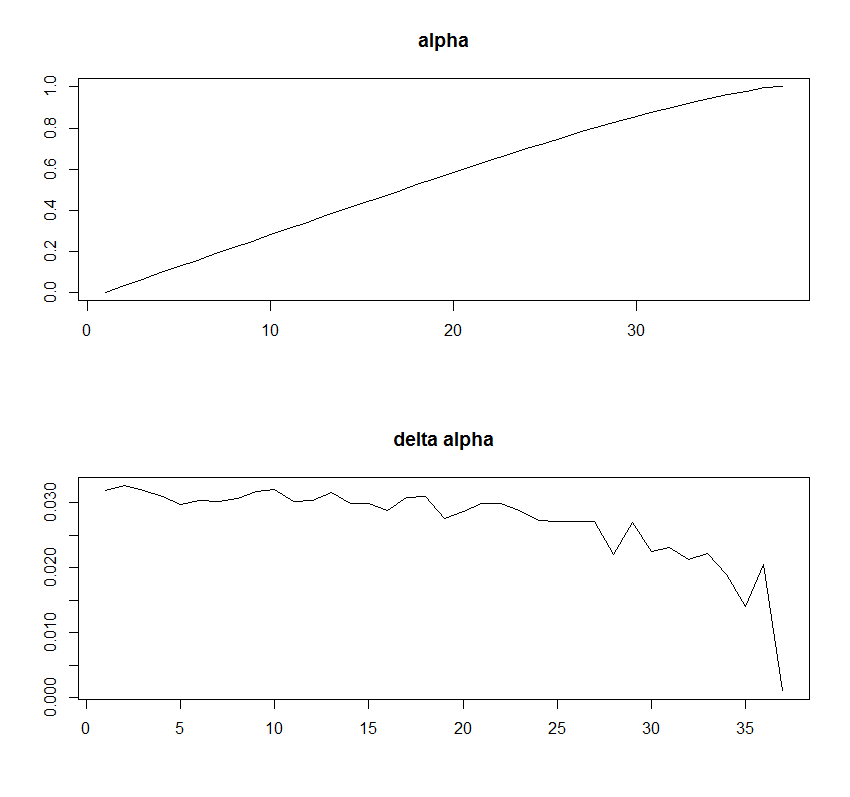
\includegraphics[width=0.6\textwidth]{figures/traj_alpha_example.png}
\end{frame}

%####################################################
\begin{frame}{Comparison with a standard Gibbs}
%####################################################

\begin{itemize}
\item 5 chains, $39\times 2000$ iterations to respect the tame  computational budget
\item Chains initialized on  $\theta^{(0)} \sim \eta_{VB}(\cdot)$
\item Convergence checked empirically
\item In the end : thining $=5$.  Sample of size $2000$. 
\end{itemize}
 
\end{frame}



%####################################################
\begin{frame}{Posterior}
%####################################################
\centering
 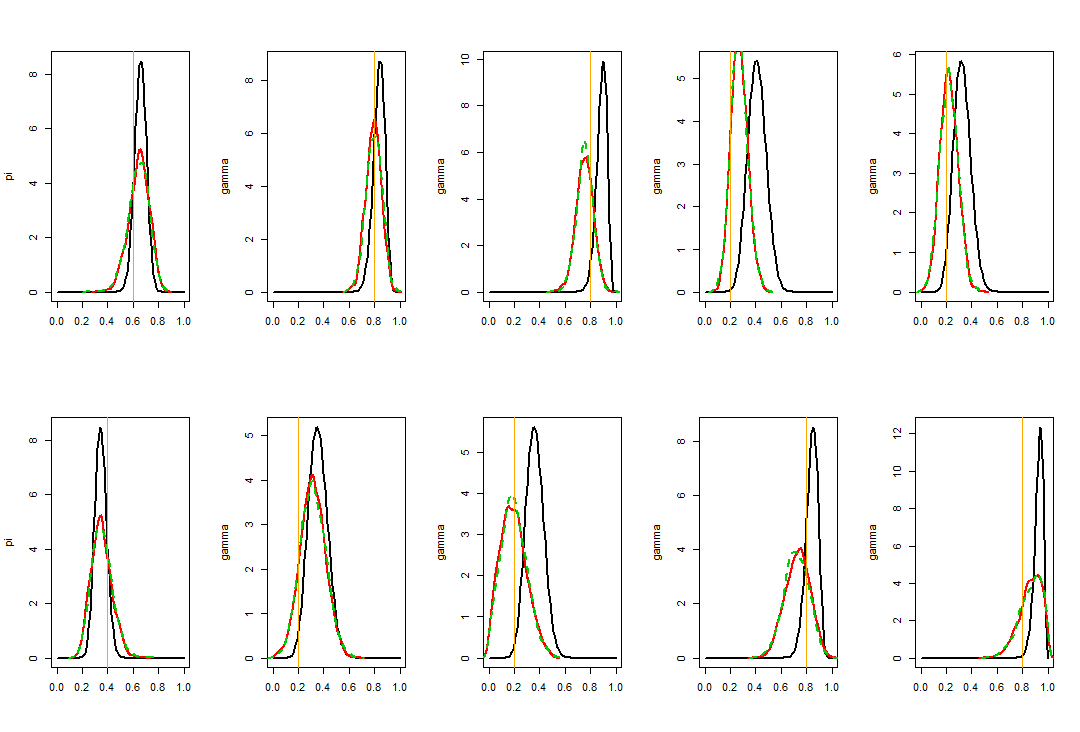
\includegraphics[width= \textwidth]{figures/post_example.png}
 
 Black : VB, Green SMC, red  MCMC
 
 See \cite{donnet2017using} for more examples
\end{frame}


